\newpage
\appendix
\onecolumn

\input appendices/scenarios.tex
\input appendices/ablation.tex
\input appendices/arch.tex

\begin{figure*}[!t]
    \centering
    \begin{subfigure}[b]{0.24\textwidth}
        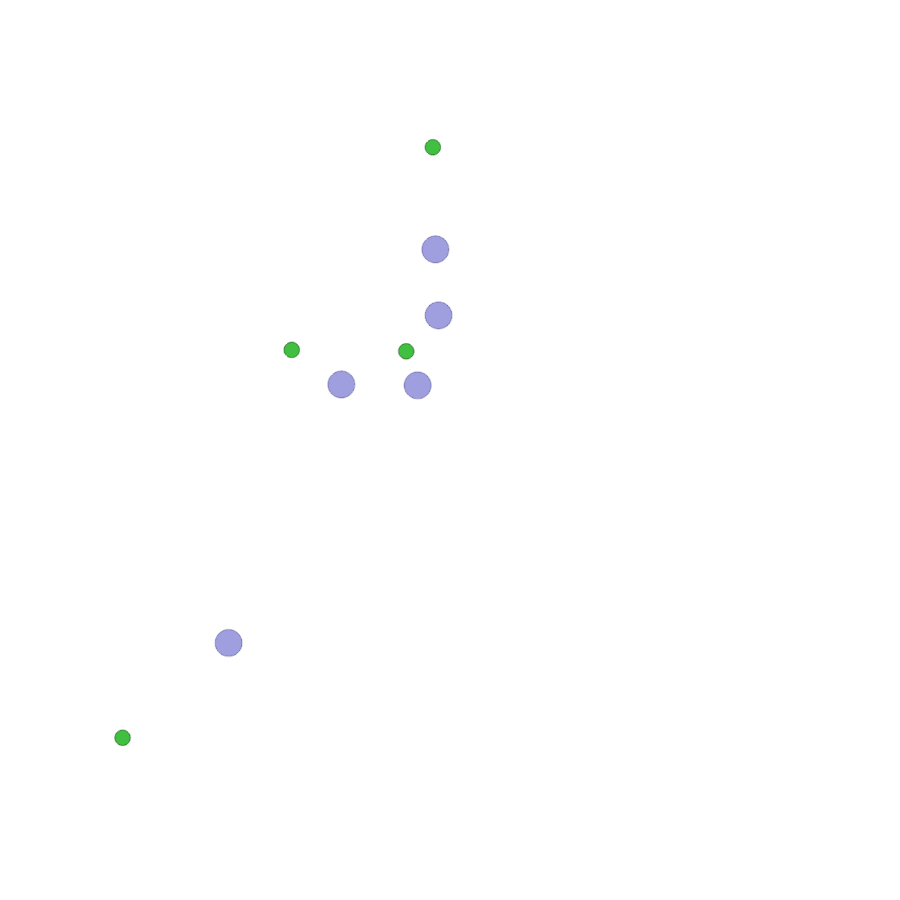
\includegraphics[width=\textwidth]{figs/dispersion.png}
        \caption{Dispersion}
        \label{fig:dispersion}
    \end{subfigure}
    \begin{subfigure}[b]{0.24\textwidth}
        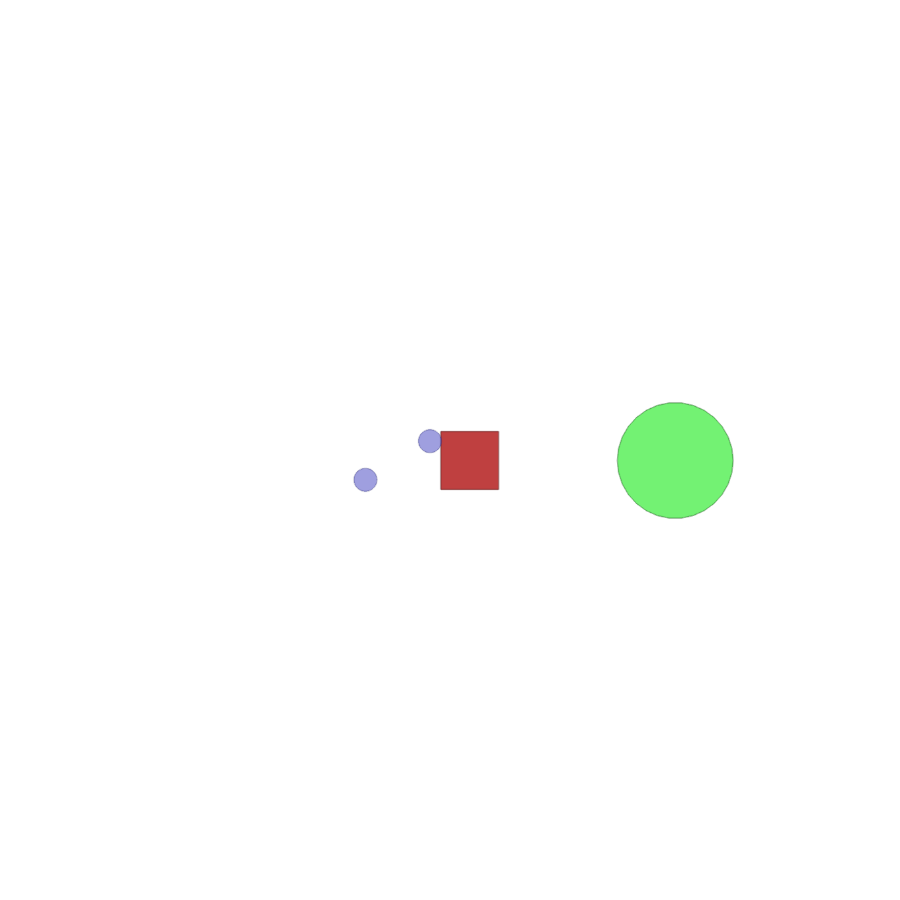
\includegraphics[width=\textwidth]{figs/transport.png}
        \caption{Transport}
        \label{fig:transport}
    \end{subfigure}
    \begin{subfigure}[b]{0.24\textwidth}
        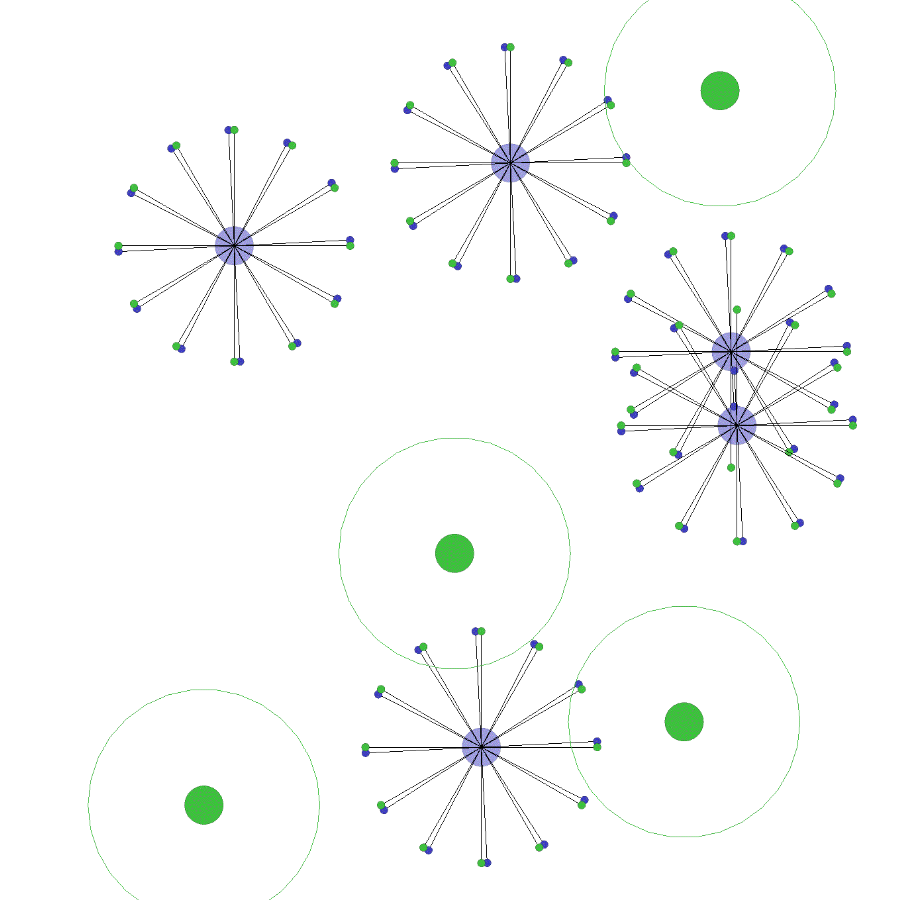
\includegraphics[width=\textwidth]{figs/discovery.png}
        \caption{Discovery}
        \label{fig:discovery}
    \end{subfigure}
    \begin{subfigure}[b]{0.24\textwidth}
        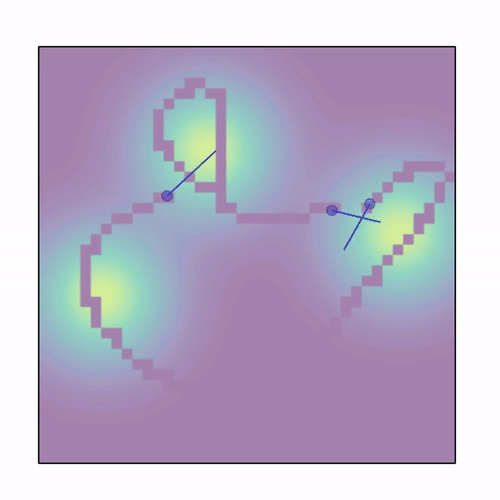
\includegraphics[width=\textwidth]{figs/sampling.png}
        \caption{Sampling}
        \label{fig:sampling}
    \end{subfigure}
    \caption{VMAS environments used in the experiments.}\label{fig:scenarios}
\end{figure*}

\begin{figure}[t]
    \centering
    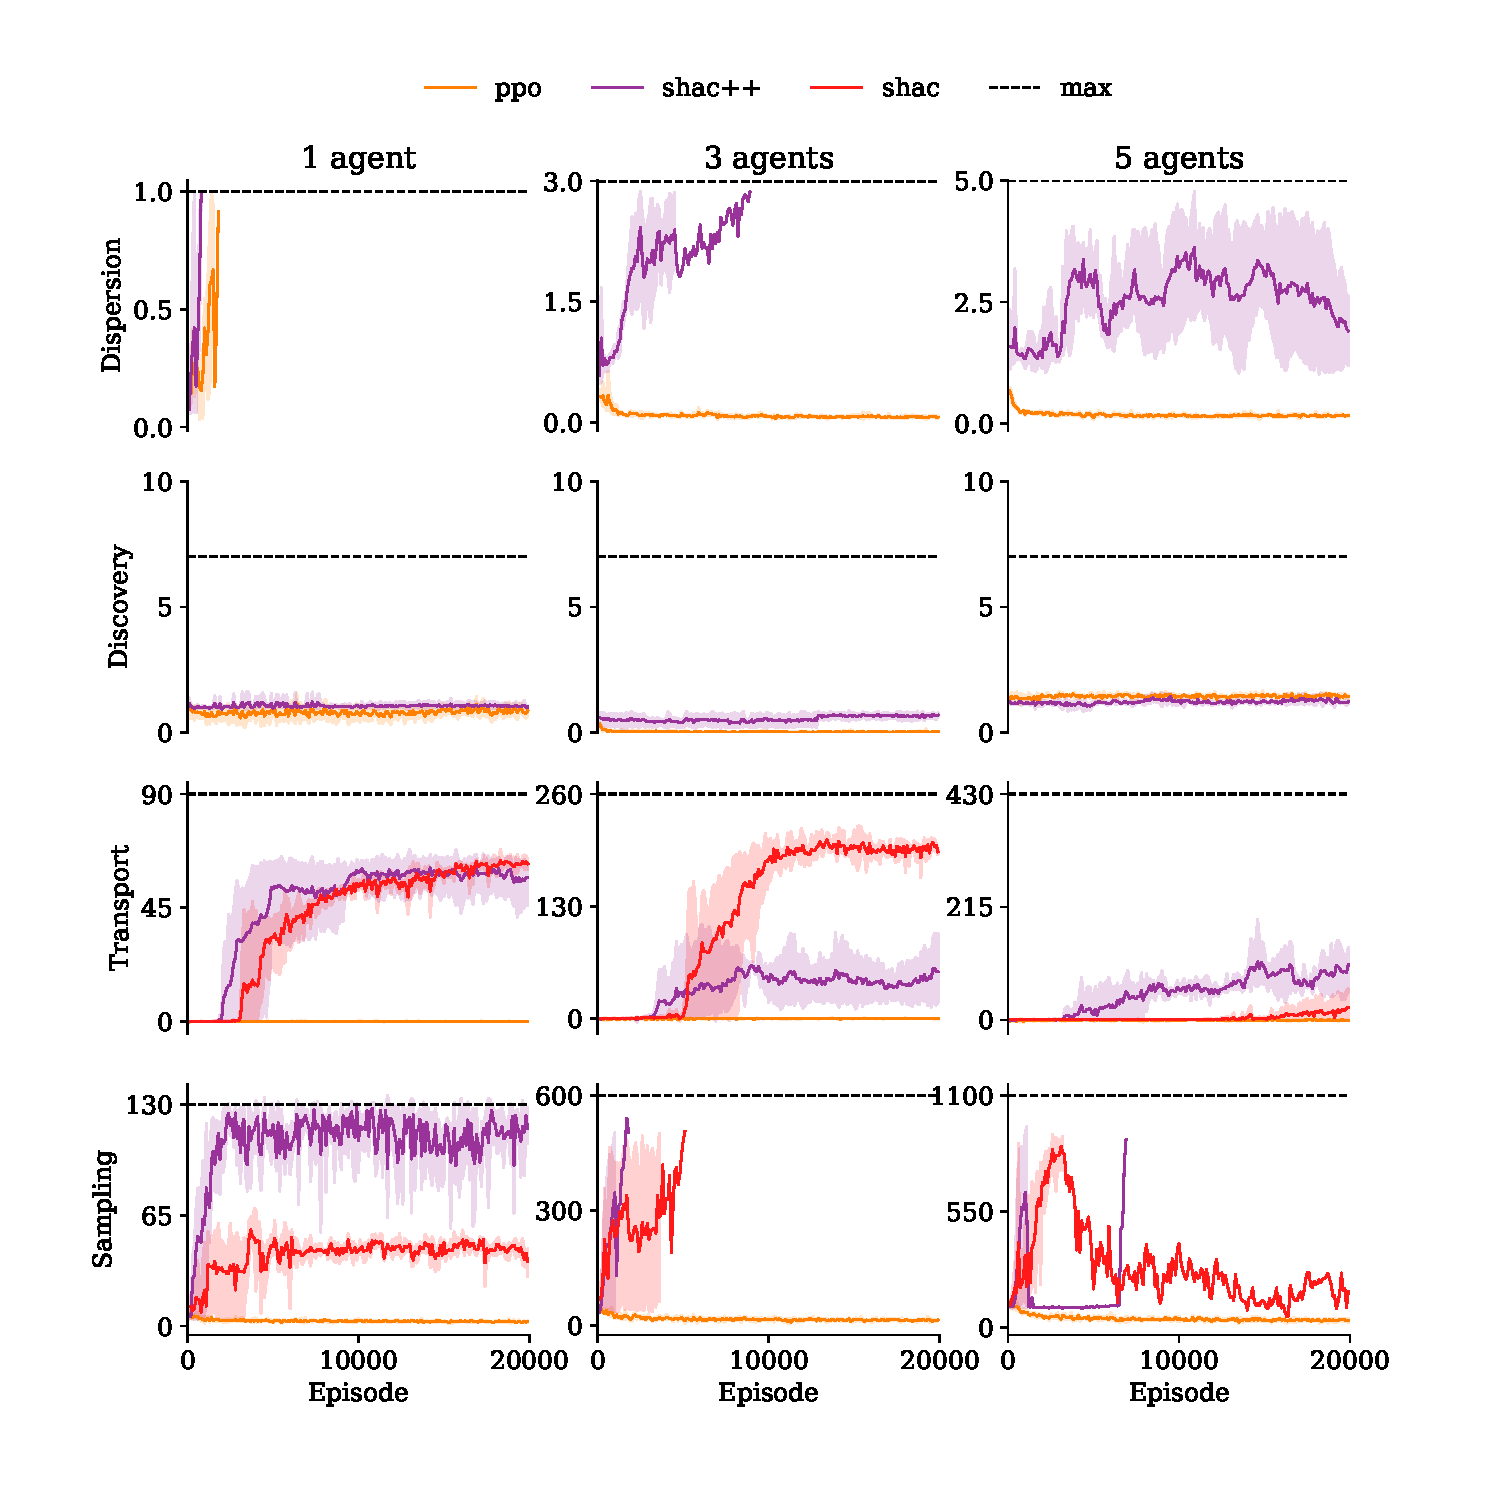
\includegraphics[width=\columnwidth]{figs/main-mlp.pdf}
    \caption{Comparison between \fname{}, PPO, and SHAC for increasing number of agents for Dispersion, Transport, Discovery, and Sampling scenarios with the MLP architecture.
    We show the mean and standard deviation of the normalized rewards across $3$ runs. For the Transformer architecture see \Cref{fig:experiments}.
    }
    \label{apx:fig:experiments-mlp}
\end{figure}

\begin{figure*}[!t]
    \centering
    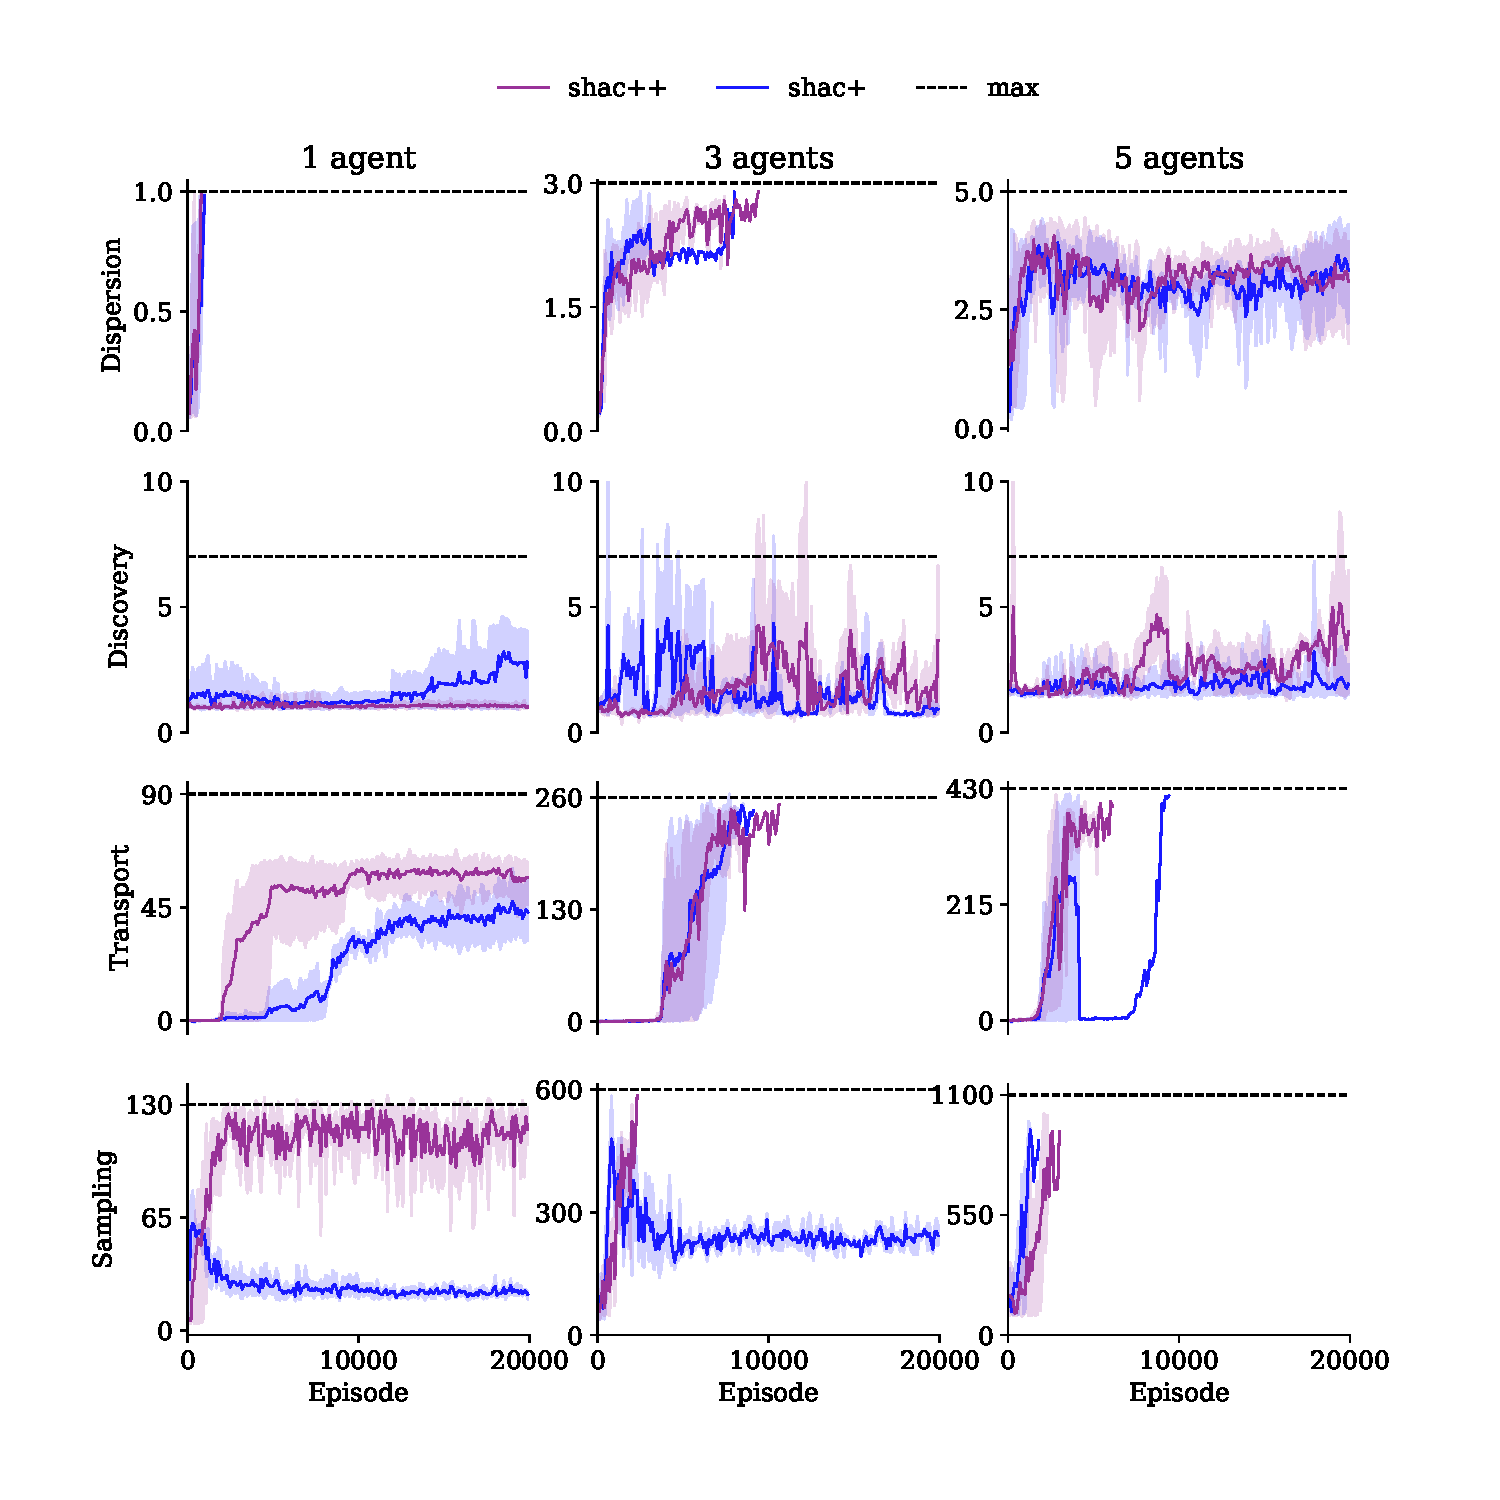
\includegraphics[width=\textwidth]{figs/ablation-transformer.pdf}
    \caption{Comparison between \fname{} with and without transition network, labelled \fnamer{}, for increasing number of agents for Dispersion, Transport, Discovery, and Sampling scenarios.}
    \label{fig:ablation}
\end{figure*}

\begin{figure}[!t]
    \centering
    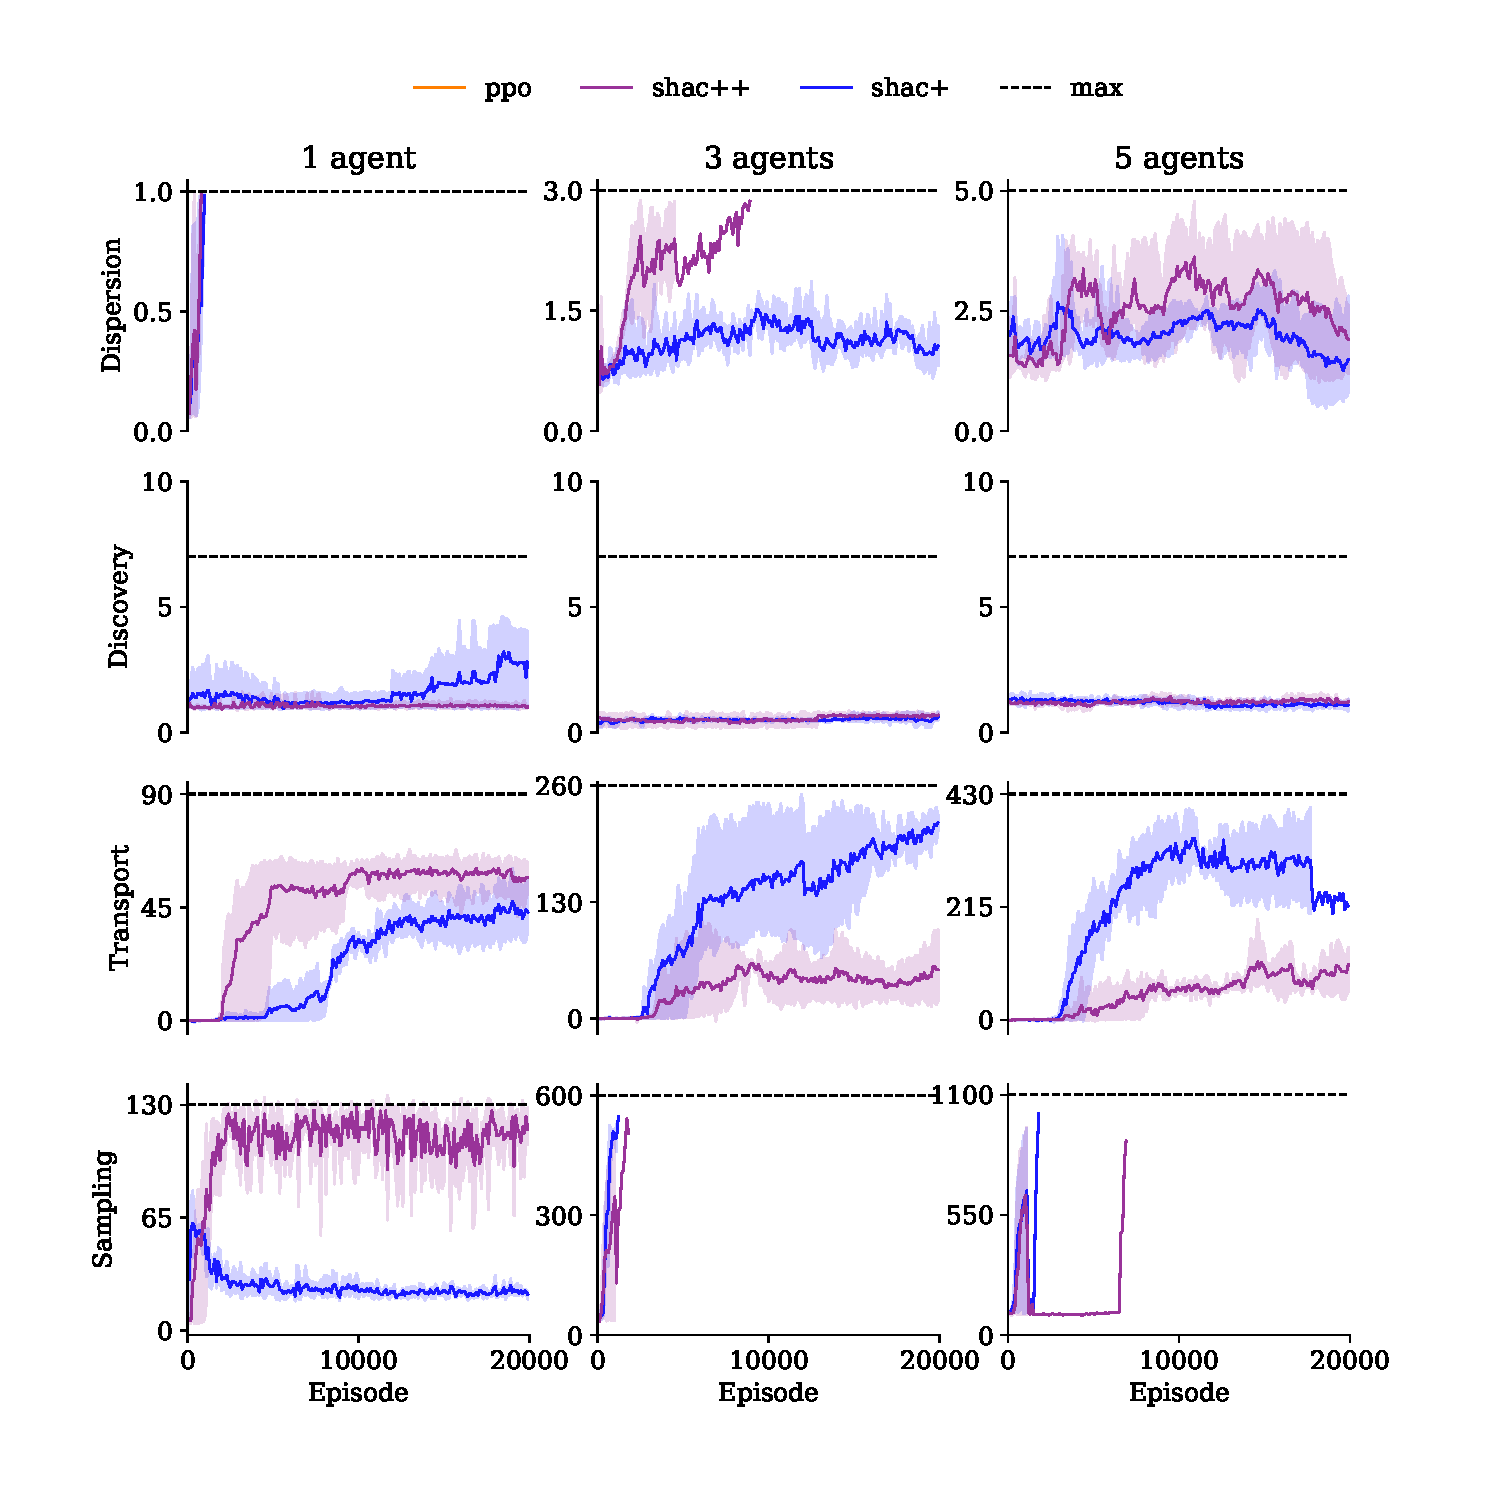
\includegraphics[width=\columnwidth]{figs/ablation-mlp.pdf}
    \caption{Comparison between \fname{} with and without transition network, labelled \fnamer{}, for increasing number of agents for Dispersion, Transport, Discovery, and Sampling scenarios.}
    \label{fig:ablation}
\end{figure}


